\section{Experiments}
\label{sec:experiments}

\subsection{Protocol}
\label{sec:dataset_setting}

We evaluate the studied HyDE-style pipeline on released IRCoT processed multi-hop QA splits under a processed local-corpus protocol. HotpotQA \texttt{test\_subsampled} is the main benchmark, and 2WikiMultihopQA \texttt{test\_subsampled} is used as a secondary generalization check. Each split contains 500 examples with supporting-title annotations and a local candidate evidence pool; corpus statistics and artifact provenance are reported in the supplement. The corpus is indexed jointly within each dataset, but the candidate paragraphs are question-tagged artifacts from the released processed data rather than a full Wikipedia collection. This setting enables paired comparison across retrieval variants on identical examples and evidence pools, but it is not a full-wiki reproduction of the original IRCoT retrieval setting.

All retrieval-reader systems use top-$k=10$ evidence passages and the same evidence-grounded short-answer reader prompt. Retrieval quality is measured by any supporting-title hit@10, all supporting-title hit@10, and mean supporting-title recall@10; answer quality is measured by normalized Exact Match (EM) and token-level F1. Because the jointly indexed corpus is constructed from released question-level candidate pools that already contain annotated support passages and semantically related distractors, we emphasize all-support hit@10 and supporting-title recall@10 over any-hit@10. The corpus records also retain \texttt{is\_supporting} flags, so Supplement Section~\ref{supp:sec:supp_evidence_case_artifacts} and Supplement Table~\ref{supp:tab:supporting_paragraph_audit} audit the same retrieval files with exact normalized title--paragraph-text matching. In the released processed splits, each annotated supporting title is associated with one supporting paragraph record, so the paragraph audit primarily verifies exact processed-record recovery rather than introducing an independent sentence-level evidence notion. This audit gives the same all-support and recall values as the title-level metrics for the audited rows listed in Supplement Table~\ref{supp:tab:supporting_paragraph_audit}, while the 500-example JSONL artifacts do not expose gold supporting sentence text for sentence-level fact coverage. The main HotpotQA table uses a MiniLM dense stack: the Sentence-Transformers implementation family introduced by Sentence-BERT \cite{reimers2019sentencebert}, the \texttt{all-MiniLM-L6-v2} MiniLM-based encoder \cite{wang2020minilm}, and a FAISS inner-product index over normalized paragraph embeddings \cite{johnson2019billion}. The BGE-base experiments are reported as stronger-encoder robustness checks rather than as a tuned replacement for the main protocol: we rerun the query-composition variants with \texttt{BAAI/bge-base-en-v1.5} \cite{xiao2023cpack} without changing prompts, top-$k$, reader settings, or the processed local-corpus protocol. Only document titles and paragraph texts are encoded for retrieval; question identifiers, supporting-evidence flags, gold answers, and evaluation metadata are excluded from retrieval representations. Qwen3.7-Max is used through an OpenAI-compatible chat-completions interface for query generation and reading with temperature-0 decoding.

The exact title--paragraph deduplication check in Supplement Table~\ref{supp:tab:dedup_retrieval_sensitivity} shows that duplicate records do not change the retrieval-side method ordering: HyDE remains the highest-scoring tested retrieval strategy under both the retained-duplicate and deduplicated local-index policies, while 2Wiki is more sensitive than HotpotQA to duplicate pressure in the joint index. Reader answers are not regenerated for the deduplicated indexes, so the sensitivity check is limited to all-support hit@10 and supporting-title recall@10.

The final HyDE-style retrieval query is question plus hypothetical passage ($q+h$); the question-only, rewritten-query, question-plus-rewritten-query, and hypothetical-only variants are reserved for the query-composition diagnostic. Prompt truncation and model/artifact constants are fixed in the scoring artifacts and documented in Supplement Table~\ref{supp:tab:configuration_provenance} and Supplement Section~\ref{supp:sec:supp_prompt_api}.

We report experiment provenance in three tiers. The primary frozen study is the original MiniLM-based HotpotQA retrieval-reader comparison: the local-corpus protocol, main lightweight baselines, HyDE query generation, matched-call direct rewriting control, top-$k=10$ retrieval budget, evidence serialization, and Qwen3.7-Max reader prompt were fixed before the canonical scoring pass for those rows. After inspecting the primary HotpotQA results, we added post-hoc robustness diagnostics rather than treating them as pre-specified primary evidence: the BGE-base stronger-encoder reproduction, gold-aware scrubbing, equal-budget query-form prompts with a 40-word target, corpus-scale and hard-negative stress tests, top-$k$ sensitivity, supporting-paragraph audit, and Qwen-Turbo fixed-evidence reader check. The equal-budget prompt templates were designed after the primary HotpotQA analysis to answer the length-versus-form concern; once written, the same 40-word target, 35--45 word instruction window, 64-token cap, and four mode templates were applied without dataset-specific modification to both HotpotQA and 2WikiMultihopQA. The 2Wiki runs are therefore used as a secondary no-retuning check for the shared diagnostic settings, not as a fully independent pre-registered benchmark. Same-split tuning is limited to the secondary verifier selector and deterministic guards, which are treated as exploratory answer-format diagnostics. Full provenance is reported in Supplement Table~\ref{supp:tab:configuration_provenance}.

We separate the reported rows into implemented lightweight baselines, mechanism controls, and heuristic controls. One-step Dense RAG, BM25 RAG, and BM25 + dense Hybrid RAG are implemented retrieval baselines under the shared local-corpus protocol. Single-query Reformulation and question-plus-rewritten-query are matched-call mechanism controls for direct rewriting, not official Rewrite-Retrieve-Read reproductions. Multi-query RAG and Rule-based Evidence-Expanded Iterative Retrieval are fixed heuristic controls for additional retrieval-query executions, not faithful implementations of published multi-query or IRCoT-style systems. HyDE-style RAG is the primary studied pipeline. The reported reader, query-generation, and diagnostic artifacts use the hosted API model string \texttt{qwen3.7-max}, and all prompt, answer, model, and analysis artifacts are frozen in Supplement Section~\ref{supp:sec:supp_prompt_api} reproducibility records.

The non-HyDE rows are implemented as fixed retrieval recipes rather than method-specific tuned systems. BM25 \cite{robertson2009probabilistic} uses lexical ranking over title--paragraph text with lowercase alphanumeric tokenization and no stopword removal. Hybrid retrieval combines the dense and BM25 top-10 ranked lists using reciprocal-rank fusion (RRF) \cite{cormack2009reciprocal}, not score interpolation. Multi-query retrieval issues three deterministic, rule-based dense queries and fuses their top-10 lists with weighted RRF; in the frozen HotpotQA artifact this changes ranking order but not the retrieved top-10 document set relative to one-step Dense RAG. Rule-based Evidence-Expanded Iterative Retrieval uses two fixed retrieval stages: a first dense retrieval, followed by three evidence-expanded dense queries built from the first-round retrieved titles and paragraph text without an additional LLM call; the final top-10 is a re-ranked union of the candidate documents. These rows are intended to isolate retrieval-budget and query-form explanations inside one reproducible protocol; they should not be read as a comprehensive public-baseline benchmark against Query2doc, Rewrite-Retrieve-Read, ReDE-RF, IRCoT, or agentic RAG systems. Full implementation parameters are reported in Supplement Table~\ref{supp:tab:baseline_implementation_parameters}.

For paired statistical comparisons, CIs are question-level paired bootstrap intervals over per-question deltas ($B=2000$, seed 13), reported as two-sided 95\% percentile intervals; paired EM tests use the two-sided exact McNemar test. The primary contrasts for interpreting the main claim are HyDE-style RAG versus one-step Dense RAG and HyDE-style RAG versus the matched-call query-reformulation mechanism control; BM25, Hybrid, Multi-query, and rule-based iterative rows are secondary context and heuristics rather than claims of superiority over all published alternatives.

\subsection{Main HotpotQA Results}
\label{sec:main_results}

HyDE-style RAG improves both evidence acquisition and answer quality on HotpotQA (Table~\ref{tab:main_results}). Compared with one-step Dense RAG, HyDE-style retrieval raises all-support hit@10 from 0.6300 to 0.8680 and mean supporting-title recall@10 from 0.8080 to 0.9280; the paired retrieval-side differences are +0.2380 [0.2000, 0.2780] for all-support hit@10 and +0.1200 [0.1010, 0.1410] for recall@10. Reader performance follows the retrieval gain, increasing from EM/F1 = 0.5940/0.7199 to 0.6840/0.8105.

\subsection{Query-Composition Diagnostics}
\label{sec:query_composition_diagnostic}

The query-composition diagnostic suggests that the larger observed gain is consistent with a combined effect of document-like generation and a larger semantic information budget, rather than the extra LLM call alone (Figure~\ref{fig:hyde_mechanism_overlap} and Table~\ref{tab:hyde_query_ablation}). A single rewritten query does not improve over question-only dense retrieval, and concatenating the original question with the rewritten query also remains near the dense baseline. In contrast, the hypothetical passage alone reaches all-support hit@10 of 0.8480 and F1 of 0.7986, while question + hypothetical passage reaches all-support hit@10 of 0.8680 and F1 of 0.8105. Paired retrieval tests strengthen this comparison: question + hypothetical passage improves all-support hit@10 over question + rewritten query by +0.2400 [0.2020, 0.2780] and mean recall@10 by +0.1250 [0.1060, 0.1470], with 123 target-only full-support cases and 3 baseline-only full-support cases.

We report the same comparison with answer-string-overlap diagnostics. A normalized diagnostic finds the gold answer in 292 of 500 HotpotQA hypothetical passages, including 252 non-trivial answer strings; the corresponding single-query reformulation overlap is 45 of 500. On the 208 HotpotQA examples without exact normalized answer overlap in the hypothetical passage, HyDE still improves Dense RAG by +0.0620 F1 [0.0170, 0.1080] (Supplement Table~\ref{supp:tab:answer_absent_subset}). Supplement Section~\ref{supp:sec:supp_answer_overlap_normalization} and Supplement Tables~\ref{supp:tab:hyde_gold_content_groups}--\ref{supp:tab:hyde_gold_content_scrubbed} add a finer automatic gold-content diagnostic: after exact-answer cases, HotpotQA examples with supporting-title or entity mentions still show a positive all-support delta of +0.1883 [0.1234, 0.2532], while the small no-identifiable-gold-content stratum ($N=32$) remains positive but has wide uncertainty. Gold-aware retrieval-only scrubbing gives the same cautionary pattern: answer-scrubbed HyDE remains above Dense on HotpotQA all-support hit@10 (0.8380 vs. 0.6300), and answer-plus-support-title-scrubbed HyDE remains above Dense (0.7800 vs. 0.6300), but both are below original HyDE (0.8680). These diagnostics weaken an exact-answer-string-only explanation while showing that generated gold entities and answer-like content are a real validity boundary. The broader interpretation of this boundary is discussed in Section~\ref{sec:discussion_limitations}.

Query-length statistics and token-matched HyDE retrieval sensitivity are reported in Supplement Table~\ref{supp:tab:query_length_matched_hyde}. The matched-call query-reformulation control equalizes query-side LLM invocations but not generated-text length or information budget. In the no-new-LLM sensitivity audit, a length-matched hypothetical-only query drops to 0.2740 all-support hit@10, while preserving the original question and matching the serialized query length to question plus rewrite gives 0.6400, close to the question-plus-rewrite baseline of 0.6280 and far below full HyDE's 0.8680. These sensitivity results motivate an independent equal-budget test rather than identifying textual form on their own.

Table~\ref{tab:equal_budget_retrieval_diagnostic} reports the stricter retrieval-only diagnostic. The same Qwen3.7-Max generator produces keyword/entity expansion, direct rewrite, question decomposition, and document-like passage forms with one call per question, the same 64-token cap, a 40-word target, BGE-base retrieval, query serialization, encoder truncation, and top-$k=10$. The realized outputs are closely length matched. Document-like passages outperform direct rewriting and question decomposition on both datasets; their comparison with keyword/entity expansion is mixed, essentially tied on HotpotQA but higher on 2Wiki. Thus, at a similar generated length and call budget, document-like organization improves over ordinary rewriting and decomposition, while the comparison with high-information keyword/entity expansion remains dataset-dependent. Because reader answers are not regenerated in this diagnostic, the mechanism conclusion remains retrieval-stage only.

We add one targeted downstream robustness check without expanding the main experiment into a reader sweep. Holding the equal-budget retrieval outputs fixed, a second hosted reader, Qwen-Turbo, re-answers the direct-rewrite, keyword/entity-expansion, and document-like top-10 evidence (Table~\ref{tab:equal_budget_reader_check}). The document-like condition improves paired F1 over direct rewrite on both datasets. Against keyword/entity expansion, it is positive on HotpotQA and tied on 2Wiki, so this fixed-evidence readout supports transfer over ordinary direct reformulation but not a universal reader-side advantage over high-information keyword expansion.

The stronger-encoder check in Table~\ref{tab:stronger_encoder_reproduction} asks a narrower question: whether the query-composition pattern persists when the MiniLM dense encoder is replaced by BGE-base without retuning the rest of the pipeline. It is not used to choose the main encoder or to report a new tuned main system. On HotpotQA with BGE-base, question-only retrieval is already strong, reaching 0.8820 all-support hit@10 and 0.8153 F1, but question + hypothetical passage still increases all-support hit@10 to 0.9200 and F1 to 0.8267. The paired deltas over question-only retrieval remain positive for all-support hit@10 (+0.0380 [0.0100, 0.0660]) and recall@10 (+0.0190 [0.0050, 0.0340]); relative to question + rewritten query, the same HyDE-style query improves all-support hit@10 by +0.0680 [0.0400, 0.0960] and F1 by +0.0212 [0.0025, 0.0410]. On 2WikiMultihopQA, question + hypothetical passage improves over question-only retrieval by +0.2700 all-support hit@10 [0.2300, 0.3120] and +0.0734 F1 [0.0444, 0.1024], and it improves over question + rewritten query by +0.3260 all-support hit@10 [0.2860, 0.3660] and +0.0978 F1 [0.0670, 0.1310]. The hypothetical-only variant is slightly higher than question + hypothetical passage on 2Wiki and marginally higher in HotpotQA answer F1, so we interpret this check as evidence that richer generated hypothetical text remains beneficial under a stronger encoder, not as evidence that one serialization or encoder setting is uniformly optimal.

Table~\ref{tab:corpus_scale_stress} adds a retrieval-only corpus-scale stress test with the same BGE-base encoder. The local baseline rows reuse the retained-duplicate BGE local-index artifacts from Table~\ref{tab:stronger_encoder_reproduction}; the expanded 50k and 100k corpora then preserve the released evaluation corpus and add exact-title--paragraph-deduplicated processed-train distractors. This separates the Table~\ref{tab:stronger_encoder_reproduction} local-index reproduction from the rounded stress-test caches, whose construction deduplicates before expansion and can therefore change small-corpus metrics. The diagnostic is still not full-wiki retrieval, but it tests whether the HyDE-style query advantage collapses when the local index contains much more noise. It does not: at 100k passages, question + hypothetical passage reaches 0.8340 all-support hit@10 on HotpotQA versus 0.6960 for question-only retrieval and 0.5960 for single-query reformulation; on 2Wiki, the corresponding values are 0.6500, 0.4180, and 0.3600. The paired all-support deltas over question-only retrieval remain positive at 100k passages on both datasets (+0.1380 [0.1000, 0.1780] on HotpotQA and +0.2320 [0.1900, 0.2760] on 2Wiki), suggesting that the retrieval effect is not only an artifact of the original small processed local corpus.

Table~\ref{tab:corpus_scale_audit} audits the same 100k stress-test construction for leakage and distractor difficulty. The random 100k HotpotQA expansion contains one added train record whose title matches a test supporting title and one near-duplicate supporting paragraph under a token-Jaccard threshold of 0.85; the corresponding 2Wiki counts are 173 and 173. Removing all added records with test supporting-title overlap leaves the released evaluation corpus intact and does not reduce the HyDE-style result: HotpotQA remains 0.8340 all-support hit@10, and 2Wiki changes from 0.6500 to 0.6520. Thus, the 100k stress-test gain is not explained by newly added gold-title leakage. The BGE similarity audit also shows that the random additions are not merely arbitrary lexical noise: the 95th percentile of each added distractor's maximum BGE similarity to any test question is about 0.60 on both datasets. A harder diagnostic that keeps the evaluation corpus but selects the most question-similar added train distractors from the audited pool raises this percentile to 0.6204 on HotpotQA and 0.6172 on 2Wiki. Under this BGE-hard 50k subset, HyDE-style retrieval still improves over question-only retrieval by +0.1460 all-support hit@10 on HotpotQA and +0.2400 on 2Wiki. This helps explain why the HotpotQA margin grows as the corpus expands: question-only retrieval loses more complete-support cases as semantically related distractors enter the index, whereas the hypothetical passage provides additional relation-bearing context that preserves more of the support ranking. The hard-negative row remains a bounded diagnostic because it selects from the processed-train 100k pool rather than from full Wikipedia.

Table~\ref{tab:topk_sensitivity} checks whether the main top-$k=10$ retrieval conclusion is a threshold artifact. We regenerate top-20 ranked lists from the frozen questions and frozen generated query text under the MiniLM+FAISS dense, BM25, direct-rewrite, and HyDE-style retrieval recipes, then rescore all-support hit and supporting-title recall at $k \in \{5,10,20\}$ without any new LLM calls. Hybrid RRF is omitted from this cutoff-sensitivity table because changing the dense/BM25 branch candidate depth can change the fused top-10 list, whereas the main Hybrid rows report the canonical top-10 fusion artifacts. HyDE-style retrieval is strongest at all three cutoffs on both datasets. On HotpotQA, all-support hit is 0.7760/0.8680/0.9080 at $k=5/10/20$, compared with 0.5060/0.6300/0.7240 for Dense and 0.4760/0.6180/0.7100 for Direct rewrite; BM25 recovers additional supports at $k=20$ but remains below HyDE-style retrieval (0.8520 versus 0.9080). On 2WikiMultihopQA, HyDE-style retrieval reaches 0.5880/0.6680/0.7140, while the strongest non-HyDE row, BM25, reaches 0.3300/0.4320/0.4740. The worst-support-rank audit gives the same interpretation: the median worst supporting-title rank is 2 for HyDE on HotpotQA and 4 on 2Wiki, compared with 5--6 and 21 for the non-HyDE rows. Thus, the observed supporting-title-completeness gain is not only a consequence of moving gold titles just inside rank 10; it also improves early support ranking and remains visible when the evidence budget is expanded to 20 retrieved passages.

\subsection{Statistical Reliability and Supporting-Title Completeness}
\label{sec:statistical_evidence_completeness}

The paired reliability checks in Supplement Table~\ref{supp:tab:hotpotqa_paired_statistics} align the answer-quality claim with example-level statistics. Relative to one-step Dense RAG, HyDE-style RAG improves EM by +0.0900 [0.0620, 0.1200] and F1 by +0.0906 [0.0634, 0.1192], with 53 wrong-to-correct and 8 correct-to-wrong EM transitions. Relative to the matched-call Single-query Reformulation baseline, HyDE improves F1 by +0.0976 [0.0690, 0.1266]. The same table shows the matching retrieval gain: +0.2500 all-support hit@10 [0.2140, 0.2860] and +0.1290 recall@10 [0.1090, 0.1500].

Supporting-title completeness buckets explain why these retrieval gains matter (Figure~\ref{fig:evidence_error_taxonomy}). Within HyDE-style RAG, full-title-support cases reach EM/F1 = 0.7396/0.8720, partial-title-support cases drop to 0.3500/0.4472, and the six no-title-support cases are all exact-match incorrect. The supplementary pooled analysis in Supplement Table~\ref{supp:tab:evidence_completeness_buckets_supp} shows the same descriptive pattern across retrieval-only method-example observations, while reusing questions across methods. We report it as descriptive support for the main pattern: supporting-title completeness, aligned with paragraph-text recovery in the processed artifacts, is a major observed bottleneck in this protocol.

% Figure 3 uses the native TikZ artwork below.
% Required packages:
% \usepackage{tikz}
% \usetikzlibrary{arrows.meta,positioning,fit,backgrounds,shapes.geometric,calc}
% \usepackage{xcolor}
% \usepackage{graphicx}

\begin{figure*}[t]
\centering
\resizebox{0.68\textwidth}{!}{%
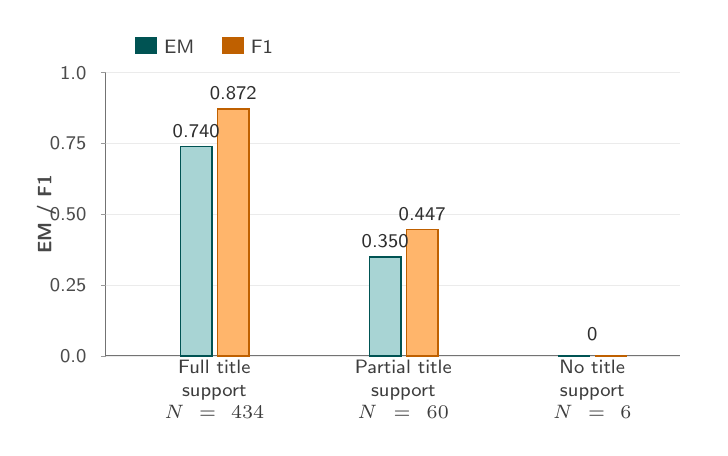
\begin{tikzpicture}[
    font=\sffamily\footnotesize,
    axis/.style={draw=black!55, line width=0.55pt},
    tick/.style={draw=black!40, line width=0.45pt},
    grid/.style={draw=black!8, line width=0.35pt},
    axislabel/.style={font=\sffamily\bfseries\scriptsize, text=black!72},
    barlabel/.style={font=\sffamily\scriptsize, align=center, text=black!76},
    value/.style={font=\sffamily\scriptsize, text=black!82},
    legend/.style={font=\sffamily\scriptsize, align=left, text=black!76}
]

% Supporting-title buckets and answer quality.
\begin{scope}[shift={(0,0)}]
    \draw[axis] (0,0) -- (7.3,0);
    \draw[axis] (0,0) -- (0,3.6);
    \foreach \y/\lab in {0/0.0,0.9/0.25,1.8/0.50,2.7/0.75,3.6/1.0} {
        \draw[tick] (-0.06,\y) -- (0,\y);
        \node[anchor=east, font=\sffamily\scriptsize, text=black!70] at (-0.12,\y) {\lab};
        \draw[grid] (0,\y) -- (7.3,\y);
    }
    \node[rotate=90, axislabel] at (-0.75,1.8) {EM / F1};

    % HyDE full title support: EM=.7396, F1=.8720
    \fill[teal!34] (0.95,0) rectangle (1.35,2.663);
    \draw[teal!65!black, line width=0.55pt] (0.95,0) rectangle (1.35,2.663);
    \fill[orange!58] (1.42,0) rectangle (1.82,3.139);
    \draw[orange!75!black, line width=0.55pt] (1.42,0) rectangle (1.82,3.139);
    \node[value] at (1.15,2.86) {0.740};
    \node[value] at (1.62,3.34) {0.872};
    \node[barlabel, text width=27mm] at (1.38,-0.42) {Full title\\support\\$N=434$};

    % HyDE partial title support: EM=.3500, F1=.4472
    \fill[teal!34] (3.35,0) rectangle (3.75,1.260);
    \draw[teal!65!black, line width=0.55pt] (3.35,0) rectangle (3.75,1.260);
    \fill[orange!58] (3.82,0) rectangle (4.22,1.610);
    \draw[orange!75!black, line width=0.55pt] (3.82,0) rectangle (4.22,1.610);
    \node[value] at (3.55,1.46) {0.350};
    \node[value] at (4.02,1.81) {0.447};
    \node[barlabel, text width=28mm] at (3.78,-0.42) {Partial title\\support\\$N=60$};

    % HyDE no title support: both metrics are zero; the small bucket is labeled without extra decimals.
    \draw[teal!65!black, line width=0.55pt] (5.75,0) -- (6.15,0);
    \draw[orange!75!black, line width=0.55pt] (6.22,0) -- (6.62,0);
    \node[value] at (6.18,0.28) {0};
    \node[barlabel, text width=25mm] at (6.18,-0.42) {No title\\support\\$N=6$};

    \node[legend, anchor=west] at (0.25,3.95) {\textcolor{teal!65!black}{\rule{8pt}{6pt}} EM \quad \textcolor{orange!75!black}{\rule{8pt}{6pt}} F1};
\end{scope}

\end{tikzpicture}%
}
\caption{Supporting-title completeness and answer quality on HotpotQA. The figure groups HyDE-style RAG examples by retrieved supporting-title completeness and reports EM/F1 within each bucket. Full title support means that all annotated supporting titles are retrieved in the top-10 evidence set. The no-title-support bucket contains only six examples and is reported descriptively. The single-annotator EM-mismatch taxonomy is reported separately in the supplement as a descriptive diagnostic.}
\label{fig:evidence_error_taxonomy}
\end{figure*}


\subsection{LLM-Call Accounting}
\label{sec:call_accounting_safety}

Structural call accounting is reported in the supplement rather than repeated as a main-text table. Dense, BM25, Hybrid, Multi-query, and the rule-based evidence-expanded iterative control each use one reader call per question, while Single-query Reformulation and HyDE-style RAG add one query-side generation call. Thus HyDE-style RAG uses 2.00 LLM calls per question and 1000 total LLM calls for the 500-example HotpotQA study. Multi-query and rule-based iterative retrieval do not add LLM calls but execute more retrieval queries per question; provider-side latency and billing are left to future cost instrumentation. The guarded canonicalization selector, guard decomposition, and single-annotator EM-mismatch taxonomy are reported only as supplemental diagnostics.

\subsection{Artifact-Grounded Case Studies}
\label{sec:case_studies}

Three examples selected from rule-filtered candidates using frozen per-example artifacts make the main mechanisms inspectable (Table~\ref{tab:qualitative_cases}). Each case is linked to existing Dense or HyDE reader outputs, supporting-title retrieval states, and HyDE overlap diagnostics.

\begin{table*}[t]
\centering
\caption{Artifact-grounded qualitative case studies emphasizing HyDE retrieval.}
\label{tab:qualitative_cases}
\scriptsize
\begin{threeparttable}
\setlength{\tabcolsep}{3pt}
\begin{tabularx}{\textwidth}{>{\raggedright\arraybackslash}p{0.17\textwidth}
                            >{\raggedright\arraybackslash}p{0.27\textwidth}
                            >{\raggedright\arraybackslash}p{0.23\textwidth}
                            >{\raggedright\arraybackslash}X}
\toprule
Case type & Question summary & Prediction / evidence state & Interpretation \\
\midrule
HyDE evidence acquisition & "Ew!" is a song by a television host born where? & Dense: United States; HyDE: Bay Ridge, Brooklyn; Gold: Bay Ridge, Brooklyn; Dense support partial (1/2); HyDE support full (2/2) & HyDE retrieves the missing supporting title without an exact normalized answer-string match in the hypothetical passage, turning a partial-evidence Dense failure into a correct answer. \\
HyDE evidence acquisition & How many films were directed by the director of Wise Blood? & Dense: I don't know; HyDE: 37; Gold: 37; Dense support partial (1/2), missing John Huston; HyDE support full (2/2) & HyDE retrieves the director page needed for the second hop and turns a partial-support Dense abstention into a correct count answer. \\
Answer-standardization boundary & Which star of Zork was also the voice of Pac-Man? & HyDE: Marty Ingels; Gold: Martin Ingerman; HyDE support full (2/2) & The reader returns the professional name Marty Ingels, whereas the benchmark gold answer uses the birth name Martin Ingerman. The two names refer to the same person, illustrating that exact-match evaluation can count semantically valid aliases as errors. \\
\bottomrule
\end{tabularx}
\begin{tablenotes}
\footnotesize
\item Cases were selected from rule-filtered candidates using frozen HotpotQA per-example artifacts: Dense and HyDE reader outputs, supporting-title states, and HyDE answer-overlap audit rows. They are illustrative rather than additional evaluation examples.
\end{tablenotes}
\end{threeparttable}
\end{table*}


The first two cases show the intended HyDE-style retrieval effect. For a question asking where the host associated with the song ``Ew!'' was born, Dense RAG retrieves only one of the two required supporting titles and answers with an over-broad country; HyDE-style retrieval recovers both supporting titles and the reader returns the exact gold location, even though the generated hypothetical passage does not contain the normalized gold answer string. For the Wise Blood counting question, Dense retrieval misses the director page and the reader abstains, while HyDE retrieves both the film and director pages and the reader returns the correct count.

The final case is an answer-standardization boundary rather than a retrieval failure. In the Zork/Pac-Man example, HyDE retrieves all supporting titles and returns the professional name ``Marty Ingels,'' while EM expects the birth name ``Martin Ingerman.'' The case illustrates why answer-format and alias diagnostics remain useful, but the main mechanism shown by the case studies is still improved evidence acquisition.

\subsection{Secondary Generalization Check}
\label{sec:2wiki_generalization}

The 2WikiMultihopQA experiment tests whether the same supporting-title completeness pattern appears on a second released processed split without retuning the reader prompt (Table~\ref{tab:2wiki_generalization}). For the primary 2Wiki evaluation, no query-generation prompt, retrieval parameter, reader instruction, or query-composition choice was selected using 2WikiMultihopQA results, so this experiment serves as an external check on the retrieval conclusion rather than as a tuning split. This split is harder for complete supporting-title retrieval: one-step Dense RAG retrieves at least one supporting title for 98.4\% of examples but all supporting titles for only 35.8\%. HyDE-style RAG raises all-support hit@10 to 0.6680 and mean recall@10 to 0.8575, and it improves reader performance to EM/F1 = 0.6620/0.7289, compared with 0.5400/0.5767 for Dense and 0.5840/0.6220 for Hybrid.

The paired 2Wiki checks in Supplement Table~\ref{supp:tab:2wiki_paired_statistics} show the same direction. Against Dense RAG, HyDE improves all-support hit@10 by +0.3100 [0.2680, 0.3520] and F1 by +0.1523 [0.1186, 0.1881]. Against Hybrid RAG, it improves all-support hit@10 by +0.2200 [0.1800, 0.2620] and F1 by +0.1069 [0.0751, 0.1399]. The 2Wiki answer-string diagnostic is reported in Supplement Section~\ref{supp:sec:supp_answer_overlap_normalization}.
